% ===================================================================
%  Week 8 — Session 1: Thresholding & region-based segmentation
% ===================================================================
\documentclass[10pt,aspectratio=169]{beamer}
% ===================================================================
%  Shared Beamer preamble for "Practical Image Processing"
%  English slides. Compile with pdfLaTeX.
% ===================================================================

\usetheme{metropolis}
\usepackage[T1]{fontenc}
\usepackage[utf8]{inputenc}
\usepackage{lmodern}
\usepackage{listings}
\usepackage{tcolorbox}
\usepackage{fontawesome5}
\usepackage{booktabs}
\usepackage{amsmath,amssymb}
\usepackage{tikz}
\usepackage{pgfplots}
\pgfplotsset{compat=1.17}
\usetikzlibrary{arrows.meta,positioning,shapes.geometric,fit,backgrounds,matrix}
\tcbuselibrary{skins,breakable}

% ---- Palette --------------------------------------------------------
\definecolor{coursePrimary}{HTML}{1B4965}   % deep blue
\definecolor{courseAccent}{HTML}{E76F51}    % coral
\definecolor{courseGood}{HTML}{2A9D8F}      % teal
\definecolor{courseBad}{HTML}{C0392B}       % red
\definecolor{courseInfo}{HTML}{2980B9}      % blue
\definecolor{codeBg}{HTML}{F5F6FA}
\definecolor{codeKw}{HTML}{8E44AD}
\definecolor{codeStr}{HTML}{2A9D8F}
\definecolor{codeCom}{HTML}{7F8C8D}

\setbeamercolor{frametitle}{bg=coursePrimary}
\setbeamercolor{progress bar}{fg=courseAccent}
\setbeamercolor{alerted text}{fg=courseAccent}
\metroset{block=fill,sectionpage=progressbar,numbering=fraction}

% ---- Code listings (Python is built into listings) -----------------
\lstdefinestyle{course}{
  backgroundcolor=\color{codeBg},
  basicstyle=\ttfamily\scriptsize,
  keywordstyle=\color{codeKw}\bfseries,
  stringstyle=\color{codeStr},
  commentstyle=\color{codeCom}\itshape,
  numberstyle=\tiny\color{codeCom},
  numbers=left, numbersep=6pt,
  showstringspaces=false, breaklines=true, breakatwhitespace=true,
  tabsize=4, columns=fullflexible,
  frame=single, framesep=4pt, rulecolor=\color{gray!30},
  keepspaces=true, upquote=true, language=Python,
}
\lstset{style=course}
\lstdefinelanguage{bash}{
  keywords={cd,pip,python,venv,source,import}, sensitive=true,
  morecomment=[l]{\#}, morestring=[b]', morestring=[b]",
}

% ---- Reusable callout boxes ----------------------------------------
\newtcolorbox{goodbox}[1][Good practice]{colback=courseGood!8,colframe=courseGood,
  fonttitle=\bfseries,title={\faCheck~#1},boxrule=0.6pt,left=4pt,right=4pt,top=3pt,bottom=3pt}
\newtcolorbox{badbox}[1][Pitfall]{colback=courseBad!8,colframe=courseBad,
  fonttitle=\bfseries,title={\faTimes~#1},boxrule=0.6pt,left=4pt,right=4pt,top=3pt,bottom=3pt}
\newtcolorbox{infobox}[1][Note]{colback=courseInfo!8,colframe=courseInfo,
  fonttitle=\bfseries,title={\faInfoCircle~#1},boxrule=0.6pt,left=4pt,right=4pt,top=3pt,bottom=3pt}
\newtcolorbox{mathbox}[1][Math]{colback=coursePrimary!6,colframe=coursePrimary,
  fonttitle=\bfseries,title={\faCalculator~#1},boxrule=0.6pt,left=4pt,right=4pt,top=3pt,bottom=3pt}

\newcommand{\keyidea}[1]{\begin{alertblock}{Key idea}#1\end{alertblock}}
\newcommand{\term}[1]{\textbf{\color{coursePrimary}#1}}
\newcommand{\code}[1]{\lstinline[basicstyle=\ttfamily\small]|#1|}

% ---- A helper to draw a small pixel grid, cells shaded by value ----
% \pixelgrid{ {10,20,120,200,240}, {30,60,130,180,230}, ... }
\newcommand{\pixelgrid}[1]{%
  \begin{tikzpicture}[font=\scriptsize,scale=0.6]
    \foreach \row [count=\ry] in {#1} {
      \foreach \val [count=\cx] in \row {
        \draw[gray,fill=coursePrimary!8] (\cx,-\ry) rectangle ++(1,-1);
        \node at (\cx+0.5,-\ry-0.5) {\val};
      }
    }
  \end{tikzpicture}}


\title{Segmentation}
\subtitle{Week 8 — Session 1: Thresholds \& regions}
\author{Practical Image Processing}
\date{Lecture 8.1 \textbullet\ 60--70 min}

\begin{document}

\maketitle

\begin{frame}{Recap \& today}
  \begin{columns}[T]
    \begin{column}{0.58\textwidth}
      \begin{itemize}
        \item Wk2/7: thresholding + morphology give clean binary shapes.
        \item \alert{Today (Session 1):} \term{segmentation} — partitioning an image
              into meaningful regions.
        \item We start where you already are (thresholds) and grow into
              \term{region-based} methods.
      \end{itemize}
    \end{column}
    \begin{column}{0.42\textwidth}
      \begin{alertblock}{DocScan milestone}
        Turn the meter photo into clean regions: page vs ink, then each digit as its
        own region --- the base for reading them.
      \end{alertblock}
    \end{column}
  \end{columns}
\end{frame}

\begin{frame}{Roadmap}\tableofcontents\end{frame}

% ==================================================================
\section{Why segmentation}
% ==================================================================

\begin{frame}{Segmentation = assign each pixel a label}
  \begin{itemize}
    \item The goal: group pixels into regions that mean something (a digit, the page, the sky).
    \item Simplest case: two labels (object / background) $=$ \term{thresholding} (Week 2).
    \item Harder: many objects, touching objects, or regions defined by colour/texture.
  \end{itemize}
  \keyidea{Segmentation is where ``pixels'' become ``objects.'' Everything downstream (counting, reading) depends on it.}
\end{frame}

\begin{frame}{A map of the methods}
  \begin{center}
  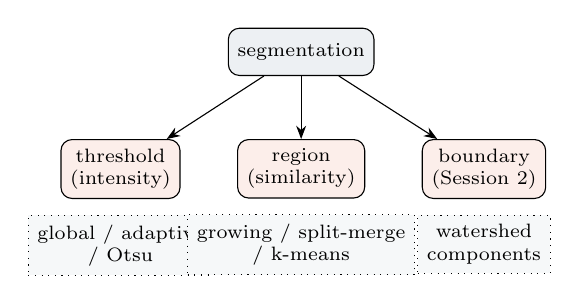
\begin{tikzpicture}[font=\scriptsize,>=Stealth,node distance=3mm and 8mm,
    b/.style={draw,rounded corners,fill=coursePrimary!8,minimum height=6mm,align=center},
    r/.style={draw,rounded corners,fill=courseAccent!12,minimum height=6mm,align=center}]
    \node[b] (seg){segmentation};
    \node[r,below left=8mm and 6mm of seg] (thr){threshold\\(intensity)};
    \node[r,below=8mm of seg] (reg){region\\(similarity)};
    \node[r,below right=8mm and 6mm of seg] (edge){boundary\\(Session 2)};
    \draw[->](seg)--(thr);\draw[->](seg)--(reg);\draw[->](seg)--(edge);
    \node[draw,dotted,below=2mm of thr,align=center,fill=coursePrimary!4]{global / adaptive\\/ Otsu};
    \node[draw,dotted,below=2mm of reg,align=center,fill=coursePrimary!4]{growing / split-merge\\/ k-means};
    \node[draw,dotted,below=2mm of edge,align=center,fill=coursePrimary!4]{watershed\\components};
  \end{tikzpicture}
  \end{center}
  \begin{itemize}
    \item Session 1 covers the left two branches; Session 2 covers boundaries.
  \end{itemize}
\end{frame}

% ==================================================================
\section{Threshold-based segmentation}
% ==================================================================

\begin{frame}{Global vs adaptive threshold --- on the meter}
  \begin{columns}[T]
    \begin{column}{0.33\textwidth}\begin{center}
      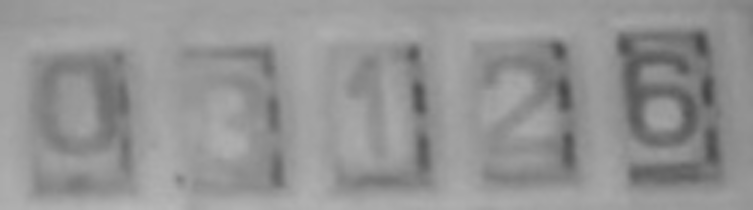
\includegraphics[width=\linewidth]{../assets/gray.png}\\{\scriptsize gray}
    \end{center}\end{column}
    \begin{column}{0.33\textwidth}\begin{center}
      
\includegraphics[width=\linewidth]{../assets/otsu.png}\\{\scriptsize global Otsu}
    \end{center}\end{column}
    \begin{column}{0.33\textwidth}\begin{center}
      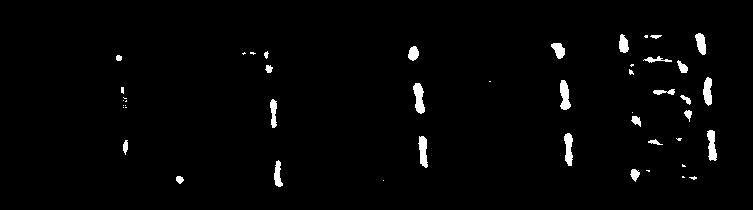
\includegraphics[width=\linewidth]{../assets/adaptive.png}\\{\scriptsize adaptive}
    \end{center}\end{column}
  \end{columns}
  \vspace{3pt}
  Otsu picks one global threshold (great for even lighting); adaptive computes a local one
  (robust to shadows). Recall Week 2 --- this is our starting point.
\end{frame}

\begin{frame}{Otsu, revisited}
  \begin{itemize}
    \item Finds the threshold that best separates the two histogram modes (max between-class variance).
    \item Works when the histogram is clearly \term{bimodal} (object vs background).
    \item Fails on: uneven lighting, more than two classes, or a unimodal histogram.
  \end{itemize}
  \begin{mathbox}
    Maximize $\sigma_B^2(t)=w_0(t)\,w_1(t)\,[\mu_0(t)-\mu_1(t)]^2$ over the threshold $t$,
    where $w_0,w_1$ are the class probabilities and $\mu_0,\mu_1$ their means.
  \end{mathbox}
\end{frame}

\begin{frame}{Otsu --- a tiny worked example}
  A 4-level image (levels 0--3) with pixel counts:
  \begin{center}\small
  \begin{tabular}{lcccc}
    \toprule
    level $i$ & 0 & 1 & 2 & 3\\
    count     & 4 & 2 & 2 & 4\\
    $p_i$     & .33 & .17 & .17 & .33\\
    \bottomrule
  \end{tabular}
  \end{center}
  Try threshold $t=1$ (class~0 = levels $\{0,1\}$, class~1 = $\{2,3\}$):
  \begin{mathbox}
    $w_0=.50,\ w_1=.50,\ \mu_0=\tfrac{0\cdot.33+1\cdot.17}{.50}=0.33,\ \mu_1=2.5$\\[2pt]
    $\sigma_B^2(1)=.50\cdot.50\cdot(2.5-0.33)^2 = 0.25\cdot 4.71 = \alert{1.18}$
  \end{mathbox}
\end{frame}

\begin{frame}{Otsu --- scanning every threshold}
  Compute $\sigma_B^2(t)$ for each candidate and keep the max:
  \begin{center}\small
  \begin{tabular}{lccc}
    \toprule
    $t$ & $w_0$ & $\mu_1-\mu_0$ & $\sigma_B^2(t)$\\
    \midrule
    0 & .33 & 1.75 & 0.68\\
    \alert{1} & .50 & 2.17 & \alert{1.18}\\
    2 & .67 & 1.75 & 0.68\\
    \bottomrule
  \end{tabular}
  \end{center}
  \begin{goodbox}
    The symmetric histogram peaks at $t=1$ --- exactly between the two modes. Otsu is
    just this scan, done over all 256 levels.
  \end{goodbox}
\end{frame}

\begin{frame}{When a single threshold fails}
  \begin{columns}[T]
    \begin{column}{0.52\textwidth}
      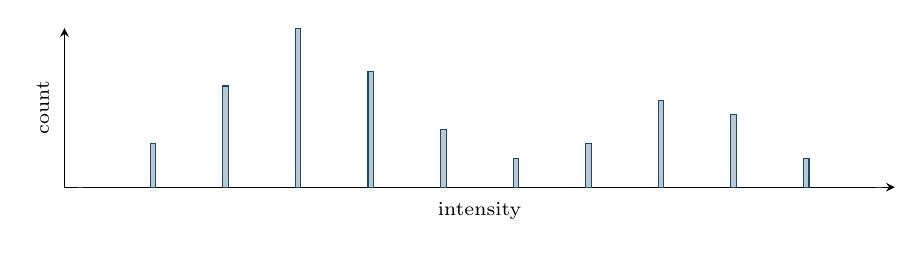
\begin{tikzpicture}
        \begin{axis}[width=\linewidth,height=3.6cm,ybar,bar width=2pt,
          xlabel={\scriptsize intensity},ylabel={\scriptsize count},
          xtick=\empty,ytick=\empty,axis lines=left,enlarge x limits=0.02]
          \addplot[draw=coursePrimary,fill=coursePrimary!30] coordinates {
            (0,2)(1,5)(2,9)(3,13)(4,10)(5,6)(6,4)(7,5)(8,8)(9,7)(10,4)(11,2)};
        \end{axis}
      \end{tikzpicture}
      {\scriptsize A shadow spreads the object mode --- no single cut separates it.}
    \end{column}
    \begin{column}{0.48\textwidth}
      \begin{badbox}
        Uneven lighting flattens the valley Otsu relies on. One global $t$ then either
        eats the shadowed text or floods the bright page.
      \end{badbox}
      Fix: compute a threshold \emph{locally}.
    \end{column}
  \end{columns}
\end{frame}

\begin{frame}{Adaptive thresholding --- how it works}
  \begin{columns}[T]
    \begin{column}{0.5\textwidth}
      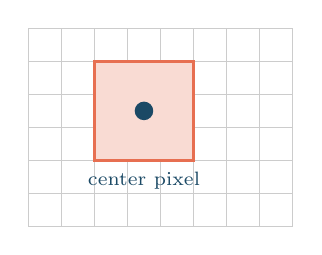
\begin{tikzpicture}[scale=0.42,font=\tiny]
        \foreach \x in {0,...,7}\foreach \y in {0,...,5}
          \draw[gray!40] (\x,\y) rectangle ++(1,1);
        \fill[courseAccent!25] (2,2) rectangle ++(3,3);
        \draw[courseAccent,very thick] (2,2) rectangle ++(3,3);
        \fill[coursePrimary] (3.5,3.5) circle (0.28);
        \node[coursePrimary] at (3.5,1.4){\scriptsize center pixel};
      \end{tikzpicture}
    \end{column}
    \begin{column}{0.5\textwidth}
      \begin{itemize}
        \item Slide a window; threshold each pixel by the \emph{local} mean (or Gaussian mean).
        \item $T(x,y)=\mathrm{mean}_{\text{block}}(x,y)-C$.
        \item Big block $\to$ smoother; small $C$ $\to$ more ink kept.
      \end{itemize}
    \end{column}
  \end{columns}
  \begin{mathbox}
    Pixel is foreground if $I(x,y) < \mathrm{mean}_{\text{block}}(x,y) - C$.
  \end{mathbox}
\end{frame}

\begin{frame}[fragile]{Adaptive threshold in code}
\begin{lstlisting}[language=Python]
import cv2
gray = cv2.imread("meter.png", cv2.IMREAD_GRAYSCALE)

# Global Otsu (one threshold for the whole image)
_, otsu = cv2.threshold(gray, 0, 255,
                        cv2.THRESH_BINARY + cv2.THRESH_OTSU)

# Adaptive: local mean over an 31x31 block, minus C=10
adap = cv2.adaptiveThreshold(gray, 255,
        cv2.ADAPTIVE_THRESH_GAUSSIAN_C,
        cv2.THRESH_BINARY, blockSize=31, C=10)
\end{lstlisting}
  \begin{itemize}
    \item \code{blockSize} must be odd; \code{C} shifts the decision brighter/darker.
  \end{itemize}
\end{frame}

\begin{frame}{Tuning adaptive threshold}
  \begin{columns}[T]
    \begin{column}{0.5\textwidth}
      \begin{badbox}
        \code{blockSize} too small $\to$ noisy speckle; too large $\to$ behaves like a
        global threshold and shadows return.
      \end{badbox}
    \end{column}
    \begin{column}{0.5\textwidth}
      \begin{goodbox}
        Start block $\approx$ the stroke width $\times$ 3, then nudge \code{C} until the
        page is clean but strokes stay connected.
      \end{goodbox}
    \end{column}
  \end{columns}
  \keyidea{Global Otsu answers ``what is the best single cut?'' Adaptive answers ``what is the best cut \emph{here}?'' Lighting decides which you need.}
\end{frame}

% ==================================================================
\section{Region-based segmentation}
% ==================================================================

\begin{frame}{Beyond thresholds}
  \begin{itemize}
    \item \term{Region growing}: start from seeds, add neighbours that are similar enough.
    \item \term{Split-and-merge}: divide the image, then merge regions that are alike.
    \item \term{Colour/k-means}: cluster pixels by colour into $k$ regions.
  \end{itemize}
  \keyidea{Thresholding uses only intensity; region methods use \emph{similarity and connectivity} --- more powerful, more parameters.}
\end{frame}

\begin{frame}{Region growing --- the idea}
  \begin{columns}[T]
    \begin{column}{0.46\textwidth}
      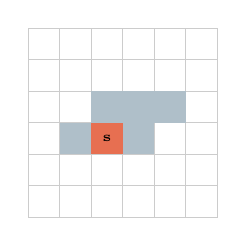
\begin{tikzpicture}[scale=0.4,font=\tiny]
        \foreach \x in {0,...,5}\foreach \y in {0,...,5}
          \draw[gray!40] (\x,\y) rectangle ++(1,1);
        \foreach \p in {(2,2),(3,2),(2,3),(3,3),(1,2),(4,3)}
          \fill[coursePrimary!35] \p rectangle +(1,1);
        \fill[courseAccent] (2,2) rectangle ++(1,1);
        \node at (2.5,2.5){\textbf{s}};
      \end{tikzpicture}
      {\scriptsize seed \textbf{s} grows into similar neighbours.}
    \end{column}
    \begin{column}{0.54\textwidth}
      \begin{enumerate}
        \item Choose seed pixel(s).
        \item Add a 4/8-neighbour if $|I_\text{nbr}-\mu_\text{region}|\le\tau$.
        \item Update the region mean; repeat until nothing is added.
      \end{enumerate}
      \begin{itemize}
        \item Grows exactly one connected region per seed.
      \end{itemize}
    \end{column}
  \end{columns}
\end{frame}

\begin{frame}{Region growing --- worked step}
  Seed at the centre ($=52$), tolerance $\tau=8$. Add a neighbour if within $\pm8$ of the region mean:
  \begin{center}
  \pixelgrid{ {50,52,90}, {51,52,88}, {49,95,92} }
  \end{center}
  \begin{itemize}
    \item Start region $=\{52\}$, mean $=52$. Neighbours $50,52,51,95$: keep $50,52,51$ ($\le\!8$), reject $95$.
    \item New mean $\approx 51.3$; its neighbour $49$ joins, $90/88/92/95$ stay out.
    \item Result: the left ``$\approx50$'' region is captured; the right bright block is a separate region.
  \end{itemize}
\end{frame}

\begin{frame}{Split-and-merge (quadtree)}
  \begin{columns}[T]
    \begin{column}{0.42\textwidth}
      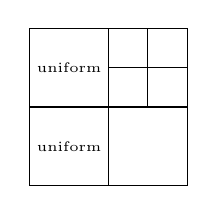
\begin{tikzpicture}[scale=0.5]
        \draw (0,0) rectangle (4,4);
        \draw (2,0)--(2,4); \draw (0,2)--(4,2);
        \draw (2,2) rectangle (4,4);
        \draw (3,2)--(3,4); \draw (2,3)--(4,3);
        \node[font=\tiny] at (1,1){uniform};
        \node[font=\tiny] at (1,3){uniform};
      \end{tikzpicture}
    \end{column}
    \begin{column}{0.58\textwidth}
      \begin{enumerate}
        \item \term{Split}: if a block is not uniform (variance $>\tau$), divide into 4.
        \item Recurse until every block is uniform.
        \item \term{Merge}: adjacent blocks that are similar become one region.
      \end{enumerate}
      \begin{itemize}
        \item Adapts detail: big blocks in flat areas, tiny blocks at edges.
      \end{itemize}
    \end{column}
  \end{columns}
\end{frame}

\begin{frame}{k-means colour segmentation --- real car}
  \begin{columns}[T]
    \begin{column}{0.5\textwidth}\begin{center}
      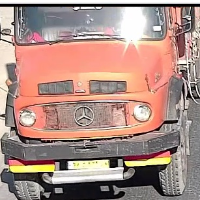
\includegraphics[width=0.85\linewidth]{../assets/car.png}\\{\scriptsize original}
    \end{center}\end{column}
    \begin{column}{0.5\textwidth}\begin{center}
      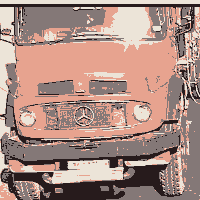
\includegraphics[width=0.85\linewidth]{../assets/car_kmeans.png}\\{\scriptsize k-means, $k$=4 colours}
    \end{center}\end{column}
  \end{columns}
  \vspace{3pt}
  \begin{itemize}
    \item Each pixel is a point in (R,G,B); k-means groups them into $k$ clusters.
    \item Replace each pixel by its cluster's colour $\rightarrow$ a segmented, posterized image.
  \end{itemize}
\end{frame}

\begin{frame}{k-means: how it works}
  \begin{enumerate}
    \item Pick $k$ initial cluster centres.
    \item Assign each pixel to the nearest centre.
    \item Recompute each centre as the mean of its pixels.
    \item Repeat 2--3 until stable.
  \end{enumerate}
  \begin{badbox}
    You must choose $k$; the wrong $k$ over- or under-segments. It also ignores \emph{position} --- only colour.
  \end{badbox}
\end{frame}

\begin{frame}{k-means --- a 1-D worked pass}
  Intensities $\{20,24,90,96\}$, $k=2$, initial centres $c_1=20,\ c_2=90$:
  \begin{mathbox}
    \textbf{Assign:} $20,24\!\to\!c_1$; \ $90,96\!\to\!c_2$.\\[2pt]
    \textbf{Update:} $c_1=\tfrac{20+24}{2}=22$, \ $c_2=\tfrac{90+96}{2}=93$.\\[2pt]
    \textbf{Re-assign:} same membership $\Rightarrow$ \alert{converged} in one pass.
  \end{mathbox}
  \begin{itemize}
    \item Final clusters: $\{20,24\}$ (dark) and $\{90,96\}$ (bright).
    \item In colour, the same runs in 3-D over (R,G,B) instead of 1-D.
  \end{itemize}
\end{frame}

\begin{frame}[fragile]{k-means in code}
\begin{lstlisting}[language=Python]
Z = img.reshape((-1, 3)).astype("float32")   # N x 3 (RGB)
crit = (cv2.TERM_CRITERIA_EPS + cv2.TERM_CRITERIA_MAX_ITER, 20, 1.0)
k = 4
_, labels, centers = cv2.kmeans(Z, k, None, crit, 10,
                                cv2.KMEANS_RANDOM_CENTERS)
seg = centers[labels.flatten()].reshape(img.shape).astype("uint8")
\end{lstlisting}
  \begin{itemize}
    \item \code{labels} is the cluster id per pixel; \code{centers} the $k$ mean colours.
    \item Run several inits (\code{attempts=10}) and keep the lowest-error one.
  \end{itemize}
\end{frame}

\begin{frame}{Choosing k}
  \begin{columns}[T]
    \begin{column}{0.5\textwidth}
      \begin{badbox}
        Too small $k$: distinct objects merge. Too large $k$: one object splits into
        colour bands (shadow vs highlight).
      \end{badbox}
    \end{column}
    \begin{column}{0.5\textwidth}
      \begin{goodbox}
        Add spatial coordinates $(x,y)$ to the feature vector so clusters stay
        spatially compact, or post-process with connected components (Session 2).
      \end{goodbox}
    \end{column}
  \end{columns}
\end{frame}

% ==================================================================
\section{In-class exercise}
% ==================================================================

\begin{frame}{\faPen~In-class exercise (10 min)}
  \begin{infobox}[Pick the threshold/region method]
  \end{infobox}
  Which Session-1 method fits each task, and what parameter matters most?
  \begin{enumerate}
    \item Dark text on an evenly lit white page.
    \item A document photographed with a shadow across half of it.
    \item Segment a photo into ``sky / road / car'' by colour.
    \item Grow the meter's dial region outward from a click at its centre.
  \end{enumerate}
\end{frame}

\begin{frame}{\faPen~Debrief}
  \begin{itemize}
    \item (1) Even lighting, bimodal $\rightarrow$ \term{Otsu}; parameter: none (auto).
    \item (2) Shadow $\rightarrow$ \term{adaptive}; parameter: \code{blockSize}, \code{C}.
    \item (3) Colour regions $\rightarrow$ \term{k-means} (or HSV colour thresholding); parameter: $k$.
    \item (4) Seeded region $\rightarrow$ \term{region growing}; parameter: tolerance $\tau$.
  \end{itemize}
  \keyidea{Match the method to the structure: intensity (threshold), lighting (adaptive), colour (k-means), or a known seed (region growing).}
\end{frame}

% ==================================================================
\section{Wrap-up}
% ==================================================================

\begin{frame}{What you can do now}
  \begin{itemize}
    \item Threshold globally (Otsu) and locally (adaptive), and know when each fails.
    \item Hand-compute Otsu's between-class variance for a small histogram.
    \item Grow a region from a seed and split/merge by uniformity.
    \item Cluster colours with k-means and reason about the choice of $k$.
  \end{itemize}
\end{frame}

\begin{frame}{Next session}
  \begin{alertblock}{Session 2 --- boundaries \& objects}
    Threshold + region methods still merge \emph{touching} objects into one blob.
    Next time: separate them with the \term{watershed}, label each with \term{connected
    components}, and measure quality with \term{IoU/Dice} --- then the week's deliverable.
  \end{alertblock}
  \begin{itemize}
    \item Bring your Otsu-vs-adaptive meter results; we build on them.
  \end{itemize}
\end{frame}

\begin{frame}[standout]
  Thresholds split by intensity, regions by similarity.\\[4pt]
  \normalsize Otsu for even light, adaptive for shadows, k-means for colour, growing from seeds.
\end{frame}

\end{document}
